\chapter{6 сентября}

\section{Организационные вопросы}

Большая часть баллов зарабатывается индивидуальными заданиями, выполняемыми в Excel --- 30 баллов. Тест с большим числом вопросов --- 20 или 25 баллов.

\section{Введение}

Теория вероятности состоит в следующем: исследуется случайная величина с заданным распределением. Математическая статистика занимается обратным --- даны данные, нужно приближенно найти числовые характеристики случайной величины и с некоторой уверенностью найти вид распределения. Матстатистика также исследует связанность случайных величин, их корреляцию. В идеале есть цель построить модель, которая по значениям одних случайных величин предсказывает другие.

Пусть проводится некоторое количество экспериментов, в ходе которых появились некоторые данные.
\begin{definition}
    \textbf{Генеральная совокупность} --- набор всех исходов проведенных экспериментов.
\end{definition}

В реальности наблюдается некоторая выборка генеральной совокупности, ибо рассматривать всю совокупность нецелесообразно.

\begin{definition}
    \textbf{Выборочная совокупность} --- исходы \underline{наблюдаемых} экспериментов.
\end{definition}

\begin{definition}
    Выборка называется \textbf{репрезентативной}, если её распределение совпадает с распределением генеральной совокупности.
\end{definition}

Выборка может быть нерепрезентативной, как в примере с ошибкой выжившего. Мы считаем, что таких ошибок у нас нет и все выборки репрезентативны, ибо исправление этих ошибок --- задача конкретной области, в которой используется матстатистика.

\begin{definition}[после опыта]
    Пусть проведено \(n\) наблюдаемых независимых экспериментов, в которых случайная величина приняла значение \(X_1, X_2 \dots X_n\). Набор\footnote{Или вектор.} этих данных называется \textbf{выборкой объема \(n\)}.
\end{definition}

\begin{definition}[до опыта]
    \textbf{Выборкой объема \(n\)} называется набор из \(n\) независимых одинаково распределенных случайных величин.
\end{definition}

Пусть имеется выборка в смысле ``после опыта'' объема \(n\). Её можно интерпретировать как следующую дискретную случайную величину:
\begin{center}
    \begin{tabular}{C|C|C|C|C|C}
        X_i & X_1         & X_2         & \dots & X_n         & \sum \\ \hline
        p_i & \frac{1}{n} & \frac{1}{n} & \dots & \frac{1}{n} & 1
    \end{tabular}
\end{center}

\textbf{Средневыборочное}:
\[\overline{X} \coloneqq \sum_{i=1}^{n} \frac{1}{n} X_i = \frac{1}{n} \sum_{i=1}^{n} X_i\]

\textbf{Выборочная дисперсия}:
\[S^2 = \sum_{i=1}^{n} (X_i - \overline{X})^2 \cdot \frac{1}{n} = \frac{1}{n} \sum_{i=1}^{n} (X_i - \overline{X})^2\]

\subsection{Выборочная функция распределения}

\[F_n^*(z) \coloneqq \frac{1}{n} \sum_{i = 1}^{n} I(X_i < z) = \frac{\mathrm{число}\ X_i \in ( - \infty, z)}{n}\]
\begin{remark}
    \(I\) --- индикатор:
    \[I(X_i < z) = \begin{cases}
            1, & X_i < z    \\
            0, & X_i \geq z
        \end{cases}\]
\end{remark}

\begin{theorem}
    \[\forall x \in \R \quad F_n^*(z) \xrightarrow[n \to \infty]{P} F(z)\]
\end{theorem}
\begin{proof}
    Заметим, что
    \[\mathbb{E} I(X_1 < z) = 1 \cdot P(X_1 < z) + 0 \cdot P(X_1 \geq z) = P(X_1 < z) = F(z)\]
    , где \(F(z)\) --- функция распределения \(X_1\). Заметим, что \(F(z) \leq 1 < \infty\), следовательно применим ЗБЧ Хинчина:
    \[F_n^*(z) = \frac{\sum_{i = 1}^{n} I(X_i < z)}{n} \xrightarrow{P} \mathbb{E} I(X_1 < z) = F(z)\]
\end{proof}
\begin{remark}
    На самом деле имеется даже равномерная сходимость по вероятности --- это теорема Гливенко-Кантелли:
    \[\sup_{z \in \R} |F_n^*(z) - F(z)| \xrightarrow[n \to \infty]{P} 0\]
\end{remark}

\section{Первоначальная обработка статданных}

Если отсортировать данные, то получим \textbf{вариационный ряд}: \(X_{(1)} \leq X_{(2)} \leq \dots \leq X_{(n)}\). Если учесть повторяющиеся экземпляры, то получим \textbf{частотный вариационный ряд}:
\begin{center}
    \begin{tabular}{C|C|C|C|C|C}
        X_{(i)} & X_{(1)}        & X_{(2)}        & \dots & X_{(k)}        & \sum \\ \hline
        n_i     & n_1            & n_2            & \dots & n_k            & n    \\ \hline
        p_i^*   & \cfrac{n_1}{n} & \cfrac{n_2}{n} & \dots & \cfrac{n_k}{n} & 1
    \end{tabular}
\end{center}

\begin{definition}
    \(h \coloneqq X_{\max} - X_{\min}\) --- \textbf{размах выборки}
\end{definition}

Допустим, что разбили интервал \((X_{\min}, X_{\max})\) на \(k\) интервалов, чаще всего одинаковой длины.\footnote{Применяются и другие разбиения, например равнонаполненное.} Тогда \(l_i = \frac{h}{k}\) --- длина каждого интервала и интервальный ряд можно заменить интервальным вариационным рядом.

\begin{center}
    \begin{tabular}{C|C|C|C|C|C|C}
        i              & l_1            & l_2            & \dots & l_k            & \sum \\
        m_i            & m_1            & m_2            & \dots & m_k            & n    \\
        \cfrac{m_i}{n} & \cfrac{m_1}{n} & \cfrac{m_2}{n} & \dots & \cfrac{m_k}{n} & 1    \\
    \end{tabular}
\end{center}
\(m_i\) --- число попавших в \(i\)-тый интервал данных.

По такой таблице можно построить \textbf{гистограмму}. На координатной плоскости построим прямоугольники c основаниями \(l_i\) и высотами \(\frac{m_i}{n l_i}\). В результате получаем ступенчатую фигуру площади \(1\), которая и называется гистограммой.

\begin{figure}[H]
    \centering
    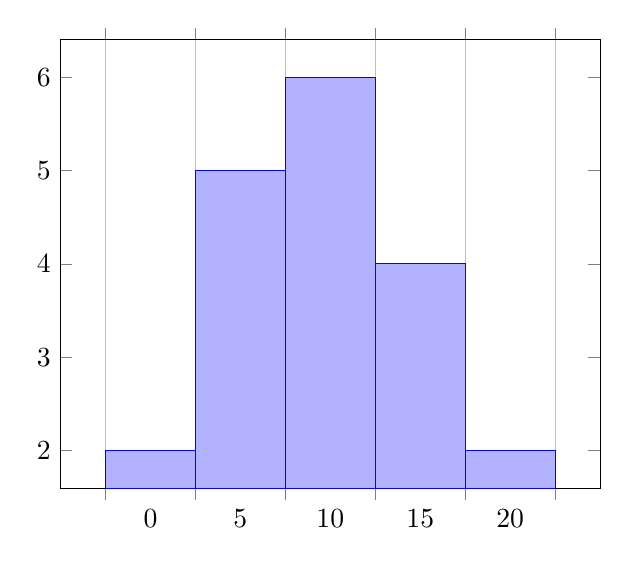
\begin{tikzpicture}
        \begin{axis}[ybar interval]
            \addplot coordinates { (0, 2) (5, 5) (10, 6) (15, 4) (20, 2) (25, 2) };
        \end{axis}
    \end{tikzpicture}
    \caption{Пример гистограммы.}
\end{figure}

\begin{theorem}
    При \(n \to \infty, k(n) \to \infty\), причем \(\frac{k(n)}{n} \to 0\), гистограмма будет стремиться к плотности распределения:
    \[\frac{m_i}{n} \xrightarrow{P} P(X_i \in l_i) = \int_{l_i} f(x)dx\]
\end{theorem}
Чаще всего число интервалов берется по формуле Стёрджесса: \(k \approx 1 + \log_2 n\). Иногда \(k \approx \sqrt[3]{n}\).

\begin{remark}
    Иногда выборка изображается в виде \textbf{полигона}: отображаются точки, соответствующие серединам интервалов и ставим точки на высоте \(\frac{m_i}{n}\).
    \begin{figure}[H]
        \centering
        \begin{tikzpicture}
            \begin{axis}
                \addplot coordinates { (0, 2) (5, 5) (10, 6) (15, 4) (20, 1) };
            \end{axis}
        \end{tikzpicture}
        \caption{Пример полигона.}
    \end{figure}
\end{remark}
